\documentclass[12pt]{article}

\usepackage[a4paper, margin=2.5cm]{geometry}
\usepackage{graphicx}
\usepackage{rotating}
\usepackage[english]{babel}
\usepackage{appendix}
\usepackage{listings}
\usepackage{url}
\usepackage{todonotes}

\graphicspath{{./resources}}
  
\title{COMP3900-H15A-capSquad - Project Proposal}
\date{\today}
\author{Daniel Latimer z5115175 \\ Connor O'Shea z5115177 \\ Kevin Chan z5113136 \\ Oliver Richards z5157383 \\ Peter Kerr z5115807} 

\begin{document}

\maketitle
\tableofcontents
\newpage

\section{Background}

\begin{figure}
    
\includegraphics[width=\textwidth]{resources/spongebob}
    \caption{Background? \cite{Laird2012}}
    \label{fig:background}
\end{figure} \todo{delete me}

\subsection{Problem Domain}
\subsection{Existing Systems}

\section{User Stories}

\subsection{Product Backlog}

The 29 user stories which make up the product backlog were grouped into three categories as described in the sections below.

\begin{figure}
    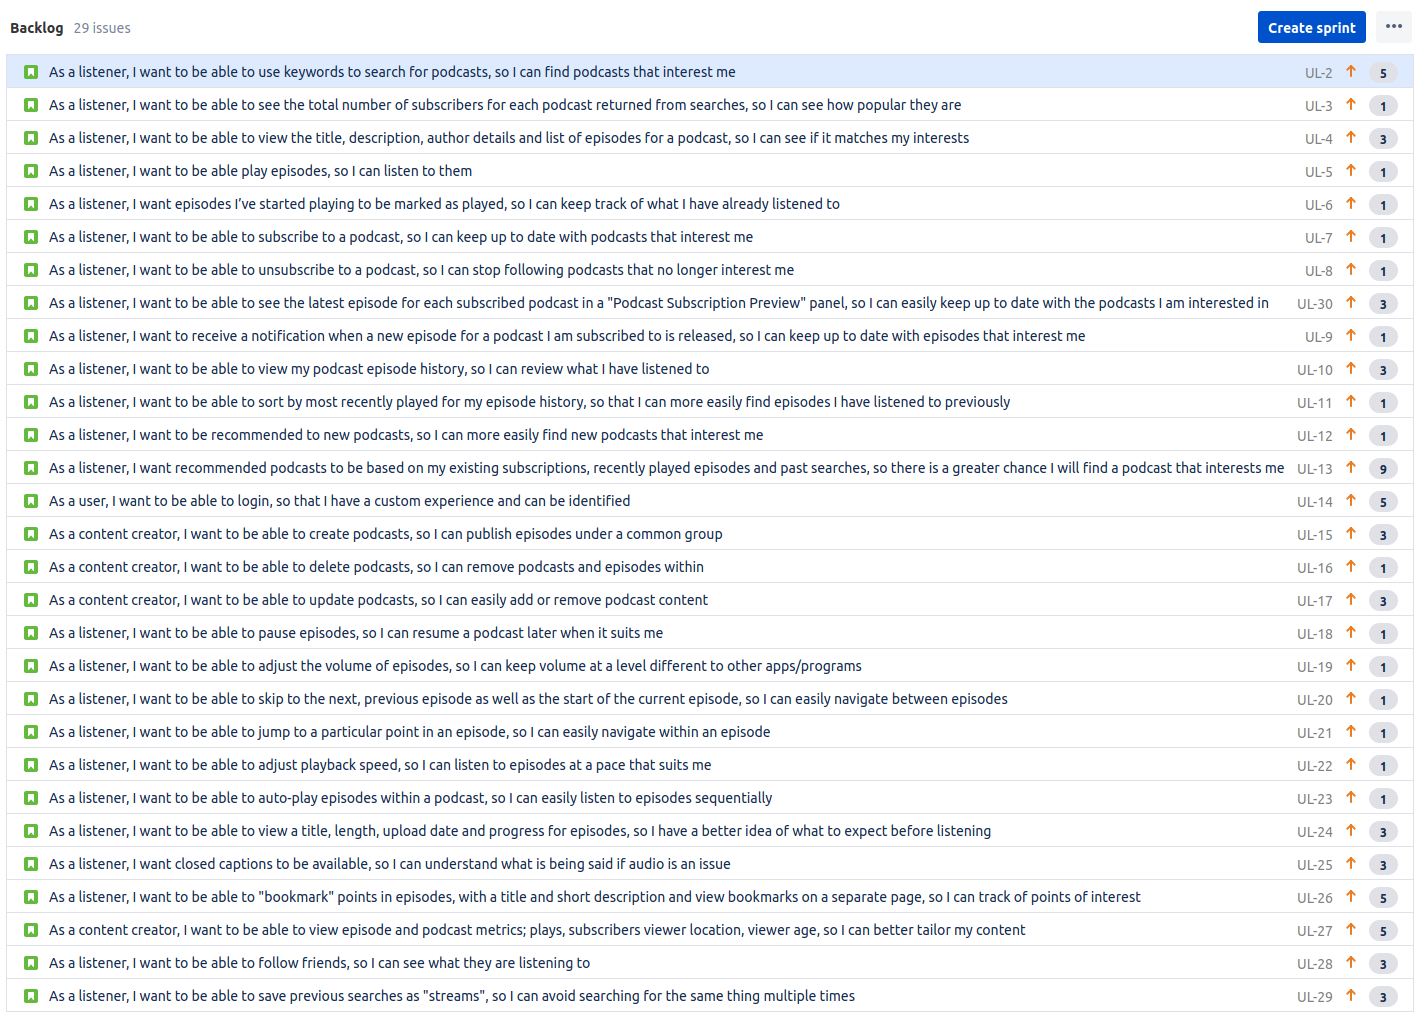
\includegraphics[width=\textwidth]{resources/backlog}
    \caption{UltraCast Backlog \cite{Laird2012}}
    \label{fig:background}
\end{figure}

\subsubsection{Project Objectives Stories}

The project objective stories were derived directly from the project objectives. The mapping of each objective to the final user story was summarised in Table XXX.

TODO format below as table

Listeners must be able to search for podcasts that interest them by keywords, resulting in a list of matching podcast titles, where the total number of subscriptions on the ultraCast platform (function described later) for each podcast is shown next to the title. 

\subsubsection{System Stories}

The system stories were designed to address common features offered by existing offerings in the same problem domain. They can be seen in Figure XXX below.

TODO add figure of system stories

\subsubsection{Novel Features Stories}

The novel feature stories were designed to create desirable features that are either uncommon or not available in other mainstream offerings in the same problem domain.

TODO stories + reason for being unique

\subsection{Sprints}
% Must have:
%   - Start + end dats of all sprints
%   - User stories in 1st sprint
%   - 

\section{Interface and Flow Diagrams}

\section{System Architecture}

The proposed system architecture can be seen in Figure \ref{fig:SysArch}.
First, we will use MongoDB to store our data, a NoSQL database that is popular for its high scalability.
This service will be interfaced with the MongoDB-Python driver, available on the MongoDB website.
Next, we will be using Flask for our web-server: a micro-framework that allows us to quickly develop an MVP solution.
Flask is written in Python, so connecting to the database via the MongoDB-Python driver should be straightforward.
Additionally, we will have a recommendation service that will generate recommended podcasts based on the users listening history.
Finally, we will have a React frontend application that will enable our users to login, search and play podcasts, and get recommendations on ones they may be interested in.
The React application and Flask application will communicate through a GraphQL API: a scalable alternative to the popular REST API.

The architecture has been designed with the final demonstration in mind, hence, the business and presentation layers are shown to be hosted on the VLab machine.
Currently, MongoDB is not supported by Debian 6 (the Linux environment on the VLab machine), so we have opted to put the data layer onto an AWS EC2 instance.

\begin{figure}
    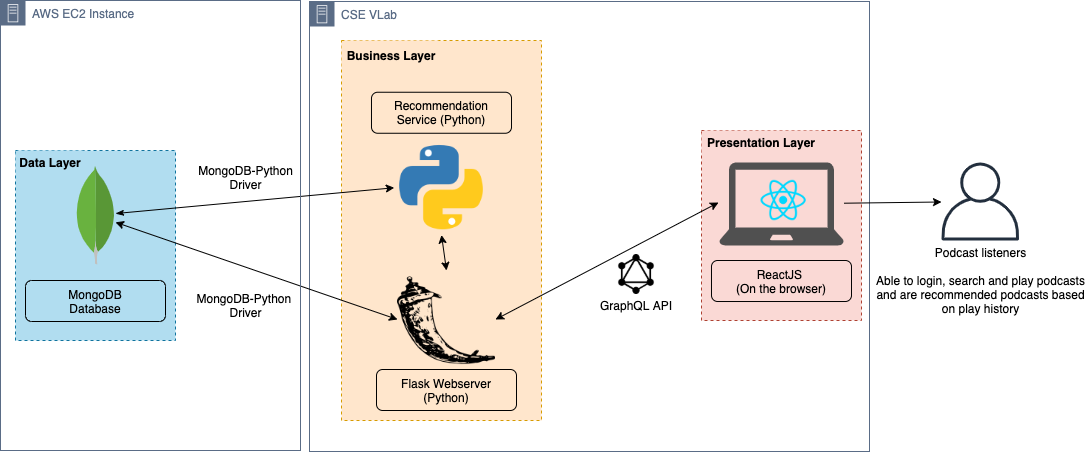
\includegraphics[width=\textwidth]{resources/SystemArchitecture}
    \caption{Proposed System Architecture}
    \label{fig:SysArch}
\end{figure}

\bibliography{library.bib}
\bibliographystyle{plain}
\end{document}
